% !TEX root = ../beamer.tex
\begin{frame}[t]
    \frametitle{DSL}
\end{frame}

\begin{frame}[t]
    \frametitle{Generated Code}
\end{frame}

\begin{frame}[t]
    \frametitle{Generator}
    
	\begin{center}   
	\begin{tikzpicture}[
		>=stealth,
		node distance = 0.75cm and 0.25cm,
		every node/.style={minimum height = 1.75em}]
		\node[draw] (dsl) {DSL\vphantom{Aq}};
		\node[draw, below = of dsl] (md2model) {MD2 Model\vphantom{Aq}};
		\draw[->] (md2model) -- node[right] {\tiny{uses}} (dsl);
	    
		\node[below = of md2model, draw] (preprocessor) {Preprocessor\vphantom{Aq}};
		\draw[->] (md2model) -- node[right] {\tiny{processed by}} (preprocessor);
		
		\node[draw, below = of preprocessor] (generator) {Generator\vphantom{Aq}};
		
		\draw[->] (preprocessor) -- node[right] {\tiny{input for}} (generator);
		
		\node[draw, below left = 0.25cm of generator] (mapapps) {map.apps source\vphantom{Aq}};
		\node[draw, below right = 0.25cm of generator] (backend) {backend source\vphantom{Aq}};
		
		\draw[->] (generator) -| node[above] {\tiny{generates}} (mapapps);
		\draw[->] (generator) -| node[above] {\tiny{generates}} (backend);
	\end{tikzpicture}
	\end{center}
\end{frame}

\begin{frame}[t]
    \frametitle{Deployment}
    
    \begin{center}   
	    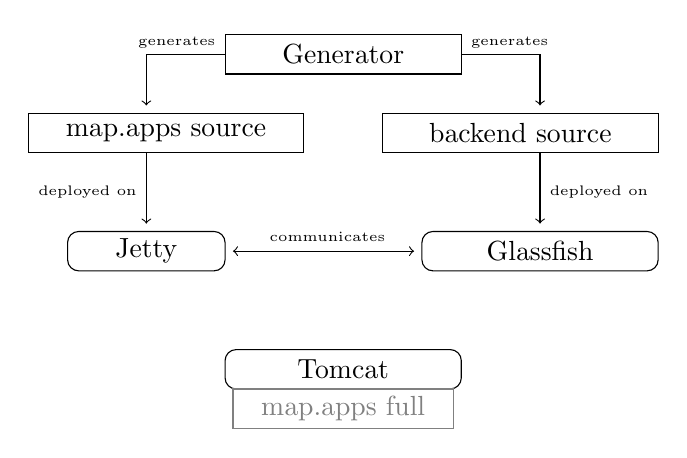
\begin{tikzpicture}
	    
	    \draw (-1.5,-4.5) rectangle (1.5,-4) node[pos=.5] {Generator};
	    
	    \draw (-4,-5.5) rectangle (-0.5,-5) node[pos=.5] {map.apps source};
	    \draw (0.5,-5.5) rectangle (4,-5) node[pos=.5] {backend source};
	    
	    \draw [->] (-1.5,-4.25) -- (-2.5,-4.25) -- (-2.5,-4.9);
	    \node [left] at (-1.5,-4.1) {\tiny{generates}};
	    \draw [->] (1.5,-4.25) -- (2.5,-4.25) -- (2.5,-4.9);
	    \node [right] at (1.5,-4.1) {\tiny{generates}};
	    
	    \draw [rounded corners] (-3.5,-7) rectangle (-1.5,-6.5) node[pos=.5] {Jetty};
	    \draw [rounded corners] (1,-7) rectangle (4,-6.5) node[pos=.5] {Glassfish};
	    \draw [rounded corners] (-1.5,-8.5) rectangle (1.5,-8) node[pos=.5] {Tomcat};
	    \draw [gray] (-1.4,-9) rectangle (1.4,-8.5) node[pos=.5] {map.apps full};
	    
	    \draw [<->] (-1.4,-6.75) -- (0.9,-6.75);
	    \node [above] at (-0.2,-6.75) {\tiny{communicates}};
	    
	    \draw [->] (-2.5,-5.5) -- (-2.5,-6.4);
	    \node [left] at (-2.5,-6) {\tiny{deployed on}};
	    
	    \draw [->] (2.5,-5.5) -- (2.5,-6.4);
	    \node [right] at (2.5,-6) {\tiny{deployed on}};
	    
	    \end{tikzpicture}
    \end{center}
\end{frame}